%! Author = Saeid Yazdani
%! Date = 12/12/2023

\section{The System-on-Chip Era}
\label{sec:soc-era}

For many years, digital and analog macros of mixed-signal integrated
circuits were limited to few analog and digital blocks
in the same package.
Furthermore, these blocks were treated as isolated areas on
the packages as a measure to prevent noise coupling from one domain to another.

The package of an \ac{IC} is the combination of a substrate, wire bonds,
and other materials to provide mechanical support.
In this context, \emph{package noise} is the undesirable electrical noise
or interference that occurs within the package of integrated circuits.

Like any other electronic circuit where electrons flow, \acp{IC} are prone to
noise and generate noise themselves.
The switching of digital circuits produces current peaks, resulting in
voltage fluctuations on the power supply lines due to the inductive behavior of
on-chip and chip-to-package interconnects \autocite{Popovich}.
In short, the noise source can be one or a combination of the following
phenomena:

\begin{itemize}[topsep=8pt,itemsep=4pt,partopsep=4pt, parsep=4pt]

    \item \textbf{\emph{Switching Noise}:} Transistors
    switch between high and low states.

    \item \textbf{\emph{Ground Bounce}:} High currents flow during
    switching events and cause voltage drops on the ground connection due to
    parasitic resistances and inductances.

    \item \textbf{\emph{Power Supply Noise}:} The \ac{IC} functionality will be
    negatively affected if the external power supply exhibits anomalies such
    as fluctuation, undershoot, or overshoot.

\end{itemize}

Package noise negatively affects the performance and functionality of \ac{IC}s
where problems such as \emph{timing jitter}, \emph{signal integrity},
and \ac{EMI} may arise.

This occurrence of noise is especially undesirable in mixed-signal
chips that contain multiple \ac{ADC} and \ac{DAC} blocks.
The digital noise produced by power and signal distribution networks through the
package can propagate to noise-sensitive analog blocks through
the chip~\autocite{Tanaka}.

Over the years, progress in \ac{CAD} tools has enabled design engineers to
reduce package noise through simulation and optimized signal routing.
Simulation allows modeling and analyzing the effects of package noise on
specific areas on the die and overall performance of \ac{SoC}s.
With the simulation results fed back into signal routing tools, the parasitic
effects and crosstalk-induced interference between different signals and blocks
can be reduced to a high degree.
Power integrity and signal analysis also help with the optimization of power and
clock distribution network within the die.
On the other hand, there are new discoveries in \ac{EMI} resistive adhesive
materials and packaging methods like \ac{TSV}, \ac{WLP} (including
fan-in, fan-out, and other variants) as well as 2.5 and 3 dimensional solutions.

Thanks to improvements in design, fabrication, and packaging technologies, noise-related
issues have been greatly reduced, making it possible to combine multiple digital and
analog blocks on the same die. This has enabled the production of compact systems
either as a single package (\ac{SoC}) or as a \ac{SiP}, where several dies are integrated
within one package to provide complete system functionality.

Compared to single-function mixed-signal \ac{IC}s, \ac{SoC}s aim to include most or all
of a system's functionality, such as processing, memory, and I/O components, and can
also incorporate mixed-signal features. Similarly, \ac{SiP} solutions let designers
combine multiple specialized \ac{IC}s and components into a single, space-efficient
package, offering flexibility while keeping the footprint small. Applications in
\ac{IoT}, automotive, and consumer electronics (smartphones, entertainment systems,
etc.) rely on \ac{SoC} and \ac{SiP} devices for their dense integration of features.
It is now common to find a single \ac{SoC} or \ac{SiP} that implements all the
functionality of a complete system. \autoref{fig:traditional-vs-modern-soc} illustrates
a comparison between a single-function mixed-signal chip and a modern \ac{SoC}.

\begin{figure}[h]
    \centering
    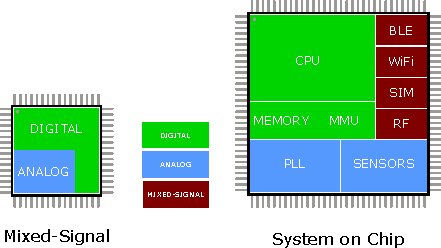
\includegraphics[scale=1.10]
    {figures/mixed-signal_vs_soc}
    \caption[Mixed-Signal v.s. System on Chip] { Comparison between a
    traditional single function mixed-signal \ac{IC} and a modern
    \ac{SoC} solutions.
    In addition to isolated analog and digital functions, an \ac{SoC} can
    host mixed-sigan cores within itself.
    }
    \label{fig:traditional-vs-modern-soc}
\end{figure}

Testing \ac{SoC}s requires \ac{ATE}s that can handle the complex and diverse
functionalities as a \ac{SoC} usually contains
functionalities distributed across multiple subsystems like \ac{CPU}s, \ac{GPU}s,
integrated memory, analog and \ac{RF} components, each requiring special
test procedures and strategies.
